% !TeX root = ../dokumentation.tex

\chapter{Roadmap}

\section{Überblick}
Nachdem die Anforderungen, die Rollenaufteilung und die Organisation des Projektes geklärt sind, geht es darum zu klären, was in den Sprints geschehen soll.
Als Orientierungshilfe werden hierbei die Anforderungen des Projektes geordnet und in Product Increments aufgeteilt.

In diesem Kontext können \acp{PI} als die geplanten größeren Versionssprünge unserer Plattform verstanden werden.
Hierbei ist es wichtig hervorzuheben, dass \acp{PI} nicht die einzelnen Sprintziele darstellen.
Diese im Voraus (mit festen zeitlichen Markern) festzulegen hätte wenig mit der im Team erzielten agilen Projektorganisation zu tun.
Vielmehr stellen die \acp{PI} des Projektes den geplanten Pfad dar, in welchem die Requirements abgearbeitet werden sollen.

\section{Product Increments}
Aus der obig erläuterten Überlegung leitet sich sie in Abbildung \ref{fig:roadmap} dargestellte Roadmap ab.
Die verschiedenen \acp{PI} sollen nun in den folgenden Abschnitten erläutert werden.

\begin{figure}
    \centering
    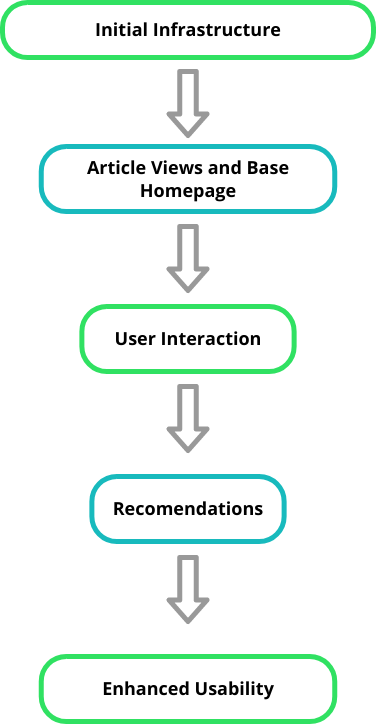
\includegraphics[width=0.3\linewidth]{roadmap.png}
    \caption{Roadmap des Projektes}
    \label{fig:roadmap}
\end{figure}

\subsection{Initial Infrastructure}
Ziel des \acp{PI} \enquote{Initial Infrastructure}\footnote{dt. Anfängliche Infrastruktur} ist es die Grundstruktur für die Plattform aufzusetzen und Workflow Elemente wie eine \ac{CI/CD} Pipeline, das Kubernetes Cluster und die initiale Servicestruktur zu erstellen.
Fragen rund um, wie die Service-Architektur und Infrastruktur aufzusetzen ist, gilt hierbei zu klären.
Am Ende dieses \acp{PI} soll das Ergebnis eine funktionsfähige Infrastruktur sein, auf welcher in kommenden Sprints entwickelt und Sprint-Ergebnisse ausgeliefert werden können.

\subsection{Article Views and Base Homepage}
Ziel des \acp{PI} \glqq Article Views and Base Homepage \grqq \footnote{dt. Artikel-Seiten und Startseite} ist es die wichtigsten Seiten der Applikation zu erstellen.
Auf Basis von Mockdaten sollen hierbei die Requirements in Richtung der Einsichtseiten von Feed und Artikel Einsichtseiten bzw. der Homepage mit vorgeschlagenen Artikeln erfüllt werden.


\subsection{User Interaction}
Ziel des \acp{PI} \enquote{User Interaction}\footnote{dt. Bernutzerinteraktion} soll das Ausbauen des User-Management Requirements sein.
Hierbei sollen sich Benutzer in die Plattform einloggen können, Feeds zur Plattform hinzufügen und abonnieren können bzw. Artikel liken und speichern können.
Da es nun einen Weg gibt Artikel zur Plattform hinzuzufügen, ist es ebenfalls Teil dieses \acp{PI} statt Mockdaten echte RSS Feeds zu verwenden.

\subsection{Recommendations}
Ziel des \acp{PI} \enquote{Recommendations}\footnote{dt. Vorschläge} ist es die Recommendations der Plattform auszubauen.
Requirements wie das Angeben von Präferenzen in Richtung Kategorien und vorgeschlagenen Feeds gilt es hier zu implementieren.
Am Ende des \acp{PI} wäre eine deutliche Verbesserung der Vorschläge für Nutzer zu erkennen.

\subsection{Enhanced Usability}
Ziel des \acp{PI} \enquote{Enhanced Usability}\footnote{dt. Verbesserte Benutzbarkeit} ist es mögliche weitere Elemente der als unrealistisch eingeschätzten Requirements zu implementieren.
Größter Fokus dieses Product Increments ist es ein Benachrichtigungssystem für Benutzer, sowie die Content-Creator Page zu implementieren.

\section{Einbringen von Sonstigen Aufgaben}
Parallel zu der eben in den \acp{PI} erläuterten technischen Implementierung des Projektes gab es ebenfalls viel fachliche Arbeit.
Aufgaben rund um Mockups und der Abgabedokumentation wurden bewusst aus der Roadmap entfernt, da diese was die Planung und Wertung angeht auf einer Meta-Ebene zum Projekt stattfanden.
Üblicherweise wurden jedoch Mockups ein \ac{PI} im Voraus bzw. die Abgabedokumentation ein (oder mehrere) \acp{PI} im Nachhinein abgearbeitet.
